\documentclass[]{book}
\usepackage{lmodern}
\usepackage{amssymb,amsmath}
\usepackage{ifxetex,ifluatex}
\usepackage{fixltx2e} % provides \textsubscript
\ifnum 0\ifxetex 1\fi\ifluatex 1\fi=0 % if pdftex
  \usepackage[T1]{fontenc}
  \usepackage[utf8]{inputenc}
\else % if luatex or xelatex
  \ifxetex
    \usepackage{mathspec}
  \else
    \usepackage{fontspec}
  \fi
  \defaultfontfeatures{Ligatures=TeX,Scale=MatchLowercase}
\fi
% use upquote if available, for straight quotes in verbatim environments
\IfFileExists{upquote.sty}{\usepackage{upquote}}{}
% use microtype if available
\IfFileExists{microtype.sty}{%
\usepackage{microtype}
\UseMicrotypeSet[protrusion]{basicmath} % disable protrusion for tt fonts
}{}
\usepackage[unicode=true]{hyperref}
\hypersetup{
            pdfborder={0 0 0},
            breaklinks=true}
\urlstyle{same}  % don't use monospace font for urls
\usepackage{color}
\usepackage{fancyvrb}
\newcommand{\VerbBar}{|}
\newcommand{\VERB}{\Verb[commandchars=\\\{\}]}
\DefineVerbatimEnvironment{Highlighting}{Verbatim}{commandchars=\\\{\}}
% Add ',fontsize=\small' for more characters per line
\usepackage{framed}
\definecolor{shadecolor}{RGB}{248,248,248}
\newenvironment{Shaded}{\begin{snugshade}}{\end{snugshade}}
\newcommand{\KeywordTok}[1]{\textcolor[rgb]{0.13,0.29,0.53}{\textbf{{#1}}}}
\newcommand{\DataTypeTok}[1]{\textcolor[rgb]{0.13,0.29,0.53}{{#1}}}
\newcommand{\DecValTok}[1]{\textcolor[rgb]{0.00,0.00,0.81}{{#1}}}
\newcommand{\BaseNTok}[1]{\textcolor[rgb]{0.00,0.00,0.81}{{#1}}}
\newcommand{\FloatTok}[1]{\textcolor[rgb]{0.00,0.00,0.81}{{#1}}}
\newcommand{\ConstantTok}[1]{\textcolor[rgb]{0.00,0.00,0.00}{{#1}}}
\newcommand{\CharTok}[1]{\textcolor[rgb]{0.31,0.60,0.02}{{#1}}}
\newcommand{\SpecialCharTok}[1]{\textcolor[rgb]{0.00,0.00,0.00}{{#1}}}
\newcommand{\StringTok}[1]{\textcolor[rgb]{0.31,0.60,0.02}{{#1}}}
\newcommand{\VerbatimStringTok}[1]{\textcolor[rgb]{0.31,0.60,0.02}{{#1}}}
\newcommand{\SpecialStringTok}[1]{\textcolor[rgb]{0.31,0.60,0.02}{{#1}}}
\newcommand{\ImportTok}[1]{{#1}}
\newcommand{\CommentTok}[1]{\textcolor[rgb]{0.56,0.35,0.01}{\textit{{#1}}}}
\newcommand{\DocumentationTok}[1]{\textcolor[rgb]{0.56,0.35,0.01}{\textbf{\textit{{#1}}}}}
\newcommand{\AnnotationTok}[1]{\textcolor[rgb]{0.56,0.35,0.01}{\textbf{\textit{{#1}}}}}
\newcommand{\CommentVarTok}[1]{\textcolor[rgb]{0.56,0.35,0.01}{\textbf{\textit{{#1}}}}}
\newcommand{\OtherTok}[1]{\textcolor[rgb]{0.56,0.35,0.01}{{#1}}}
\newcommand{\FunctionTok}[1]{\textcolor[rgb]{0.00,0.00,0.00}{{#1}}}
\newcommand{\VariableTok}[1]{\textcolor[rgb]{0.00,0.00,0.00}{{#1}}}
\newcommand{\ControlFlowTok}[1]{\textcolor[rgb]{0.13,0.29,0.53}{\textbf{{#1}}}}
\newcommand{\OperatorTok}[1]{\textcolor[rgb]{0.81,0.36,0.00}{\textbf{{#1}}}}
\newcommand{\BuiltInTok}[1]{{#1}}
\newcommand{\ExtensionTok}[1]{{#1}}
\newcommand{\PreprocessorTok}[1]{\textcolor[rgb]{0.56,0.35,0.01}{\textit{{#1}}}}
\newcommand{\AttributeTok}[1]{\textcolor[rgb]{0.77,0.63,0.00}{{#1}}}
\newcommand{\RegionMarkerTok}[1]{{#1}}
\newcommand{\InformationTok}[1]{\textcolor[rgb]{0.56,0.35,0.01}{\textbf{\textit{{#1}}}}}
\newcommand{\WarningTok}[1]{\textcolor[rgb]{0.56,0.35,0.01}{\textbf{\textit{{#1}}}}}
\newcommand{\AlertTok}[1]{\textcolor[rgb]{0.94,0.16,0.16}{{#1}}}
\newcommand{\ErrorTok}[1]{\textcolor[rgb]{0.64,0.00,0.00}{\textbf{{#1}}}}
\newcommand{\NormalTok}[1]{{#1}}
\usepackage{longtable,booktabs}
\usepackage{graphicx,grffile}
\makeatletter
\def\maxwidth{\ifdim\Gin@nat@width>\linewidth\linewidth\else\Gin@nat@width\fi}
\def\maxheight{\ifdim\Gin@nat@height>\textheight\textheight\else\Gin@nat@height\fi}
\makeatother
% Scale images if necessary, so that they will not overflow the page
% margins by default, and it is still possible to overwrite the defaults
% using explicit options in \includegraphics[width, height, ...]{}
\setkeys{Gin}{width=\maxwidth,height=\maxheight,keepaspectratio}
\IfFileExists{parskip.sty}{%
\usepackage{parskip}
}{% else
\setlength{\parindent}{0pt}
\setlength{\parskip}{6pt plus 2pt minus 1pt}
}
\setlength{\emergencystretch}{3em}  % prevent overfull lines
\providecommand{\tightlist}{%
  \setlength{\itemsep}{0pt}\setlength{\parskip}{0pt}}
\setcounter{secnumdepth}{5}
% Redefines (sub)paragraphs to behave more like sections
\ifx\paragraph\undefined\else
\let\oldparagraph\paragraph
\renewcommand{\paragraph}[1]{\oldparagraph{#1}\mbox{}}
\fi
\ifx\subparagraph\undefined\else
\let\oldsubparagraph\subparagraph
\renewcommand{\subparagraph}[1]{\oldsubparagraph{#1}\mbox{}}
\fi

\author{}
\date{\vspace{-2.5em}}

\begin{document}

{
\setcounter{tocdepth}{1}
\tableofcontents
}
\chapter{Syllabus}\label{syllabus}

\section{Instructor Information}\label{instructor-information}

Instructor: Dr.~Amy Hurford\\
Office: Teaching remotely\\
Email: \href{mailto:ahurford@mun.ca}{\nolinkurl{ahurford@mun.ca}}\\
WebEx: \url{https://mun.webex.com/meet/ahurford}\\
Course website: \url{https://ahurford.github.io/math-4190/}

Availability: I will try to reply to emails within 24 hours (excluding
evenings, weekends and holidays). I am always available during the
lecture times. Please email to request a meeting for a different time.
Please check my \href{https://amyhurford.weebly.com/}{schedule} and
suggest a time I am free that works for you.

\section{Course Information}\label{course-information}

TR 2-3.15pm meet on WebEx

Course description:\\
MATH 4190 Mathematical Modelling is intended to develop students' skills
in mathematical modelling and competence in oral and written
presentations. Case studies in modelling will be analyzed. Students will
develop a mathematical model and present it in both oral and report
form.

Course format:\\
For the first 7 weeks of class, each week you will have an assignment to
complete. There will not be lectures, but there may be required readings
(ideally to be completed before class). For the next 5 weeks, during
class time you should work on your final project. During the last week
of class each student will do an oral presentation of their final
project. During classtime, I will be available on WebEx to help you with
your assignments, to answer your questions, or to advise you regarding
your final project. If you are not able to make it to class, but require
help, please email me to set up an appointment.

Course expectations:\\
Any students that are disruptive, violating university policies, or
acting in a potentially unsafe way will be warned and asked to
leave.\\[2\baselineskip]Learning goals:\\
This course will teach you how to derive, parameterize, and interpret
your own mathematical models with an emphasis on `hands-on' modelling
experience.

Required Text and Resources:\\
The ebook at \url{https://ahurford.github.io/math-4190/} is the text for
the course. This ebook will refer you to any other readings that will be
either publically available or available via the MUN library. Class
announcements and submission of your assignments will occur through
BrightSpace.

\section{Method of Evaluation}\label{method-of-evaluation}

\begin{itemize}
\tightlist
\item
  7 assignments (equal weighting) - 35\%
\item
  Oral presentation (week of April 5) - 15\%
\item
  Written project (due Monday April 12 at 9am) - 50\%
\end{itemize}

See Section \ref{final-project} for expectations regarding the final
project.

Late assignments, labs, and missed midterms, and final exams will be
accommodated as described by University Regulation 6.7.3 and 6.7.5 (see
\url{https://www.mun.ca/regoff/calendar/sectionNo=REGS-0474} for
Regulations).

\section{Additional Policies}\label{additional-policies}

\subsection{Accommodation of students with
disabilities}\label{accommodation-of-students-with-disabilities}

Memorial University of Newfoundland is committed to supporting inclusive
education based on the principles of equity, accessibility and
collaboration. Accommodations are provided within the scope of the
University Policies for the Accommodations for Students with
Disabilities see \url{www.mun.ca/policy/site/policy.php?id=239}.
Students who may need an academic accommodation are asked to initiate
the request with the Glenn Roy Blundon Centre at the earliest
opportunity (see \url{www.mun.ca/blundon} for more information).

\subsection{Academic misconduct}\label{academic-misconduct}

Students are expected to adhere to those principles, which constitute
proper academic conduct. A student has the responsibility to know which
actions, as described under Academic Offences in the University
Regulations, could be construed as dishonest or improper. Students found
guilty of an academic offence may be subject to a number of penalties
commensurate with the offence including reprimand, reduction of grade,
probation, suspension or expulsion from the University. For more
information regarding this policy, students should refer to University
Regulation 6.12.

\subsection{Equity and Diversity}\label{equity-and-diversity}

A safe learning environment will be provided for all students regardless
of race, colour, nationality, ethnic origin, social origin, religious
creed, religion, age, disability, disfigurement, sex (including
pregnancy), sexual orientation, gender identity, gender expression,
marital status, family status, source of income or political opinion.

You should not photograph or record myself, teaching assistants, or
other students in the class without first obtaining permission.
Accommodation will be made for students with special needs.

The sound should be turned off on phones and computers during class.

\section{Additional Supports}\label{additional-supports}

Resources for additional support can be found at:

\begin{itemize}
\item
  \url{www.mun.ca/currentstudents/student/}
\item
  \url{https://munsu.ca/resource-centres/}
\end{itemize}

\section{Tentative course schedule}\label{tentative-course-schedule}

The course schedule is found in the toolbar of the class materials, see
\url{https://ahurford.github.io/math-4190/}.

The last day to drop the course without academic prejudice is Monday
March 8.

\chapter{A1. Tues Jan 12: What is a mathematical
model?}\label{a1.-tues-jan-12-what-is-a-mathematical-model}

\emph{Assignment 1, Q1-4: to be handed in on Brightspace by Tues Jan 19
at 2pm.}

\begin{center}\rule{0.5\linewidth}{0.5pt}\end{center}

\section{Questions A1-1}\label{questions-a1-1}

\begin{enumerate}
\def\labelenumi{\arabic{enumi}.}
\item
  What is a mathematical model? Give the citation for your answer in the
  style of the Bulletin of Mathematical Biology. This citation must be
  to a book (i.e., from the MUN library, or another an article from the
  peer-reviewed literature). {[}2 marks{]}
\item
  Usually statistical models such as a linear regression satisfy my
  defintion of a mathematical model. Given your definition in 1., would
  a linear regression meet the requirements for a mathematical model?
  {[}1 mark{]}
\item
  Per your answer to 1., give an example of something that is a model,
  but not a mathematical model. {[}1 mark{]}
\item
  List some types of equations that are commonly used as models. {[}1
  mark{]}
\end{enumerate}

While the definition of a mathematical model is quite broad, in keeping
with the pre-requisites for this class, we will emphasize models from
dynamical systems throughout this course.

You may search the MUN library online holdings to find a book or
peer-reviewed article to answer the above questions. Alternatively, you
may use one of the resources below:

Bliss et al. 2014
\href{https://m3challenge.siam.org/sites/default/files/uploads/siam-guidebook-final-press.pdf}{Math
modeling: getting started and getting solutions}

Otto and Day 2009.
\href{https://ebookcentral-proquest-com.qe2a-proxy.mun.ca/lib/MUN/detail.action?docID=768551}{A
biologists guide to mathematical modelling}

\href{https://link-springer-com.qe2a-proxy.mun.ca/book/10.1007\%2F978-3-030-44541-6}{A
primer on mathematical modelling} (the chapters can be downloaded for
free)

\chapter{A1. Thurs Jan 14: Getting
started}\label{a1.-thurs-jan-14-getting-started}

\emph{Assignment 1, Q5-6: to be handed in on Brightspace by Tues Jan 19
at 2pm.}

\begin{center}\rule{0.5\linewidth}{0.5pt}\end{center}

When deriving a mathematical model, some practical advice is:

\begin{enumerate}
\def\labelenumi{\alph{enumi}.}
\tightlist
\item
  Modifying an existing model to suit your purposes is often a good
  approach; and\\
\item
  The units in the terms of your model need to be consistent.\\
\end{enumerate}

We would like to derive a mathematical model for the following:

\emph{Cooling beer in the freezer}\\
Room temperature beer can be cooled down by putting it in the freezer.
If left too long, the beer will freeze and burst the glass making it
undrinkable. How long can the beer be left in the freezer?

Read Box 2.1 on p30-31 of
\href{https://ebookcentral-proquest-com.qe2a-proxy.mun.ca/lib/MUN/detail.action?docID=768551}{A
biologists guide to mathematical modelling}.

Step 1 of the modelling process has been completed because the question
has been provided. Next, we will skip to Step 4. Read about the
\emph{cooling cup of coffee} model below. We can borrow the
\emph{cooling cup of coffee} model to use as our model for the
\emph{cooling beer in the freezer} question.

\section{The cooling cup of coffee}\label{the-cooling-cup-of-coffee}

The following is taken from Barnes \& Fulford (2002), section 9.1-9.2
starting of p218.

We would like to know how long it will take a 60\(^\circ\)C cup of
coffee to drop to 40\(^\circ\)C. To develop the model, we assume the cup
of coffee is a uniform temperature throughout. The cup of coffee will
cool as heat energy from the coffee is lost to its surroundings, which
are at a lower temperature. Note that temperature is measured in degrees
Celsius, while heat is measured in Joules or Watts (Joules per second).

From physics, the equation for the change in the heat content of coffee,
\(Q_{hc}\) (in Watts) is,

\begin{equation}
Q_{hc} = cm \frac{dU(t)}{dt},
\end{equation}

where \(c\) is the heat specific constant (measured in Joules per degree
Celcius per kilogram), \(m\) is the mass of the material being heated or
cooled (in kilograms), and \(U(t)\) is the temperature in Celcius.

Also, from physics the rate of heat exchange of an object which is
hotter than its surroundings, \(Q_{cs}\), (in Watts) is,

\begin{equation}
Q_{cs} = hS(U(t)-u_s),
\end{equation}

where \(h\) is the constant of convective heat transfer (in Watts per
\(m^2\) per degree Celcuis), \(S\) is the surface area from which heat
is lost, \(U(t)\) is the temperature of the object and \(u_s<U(t)\) is
the temperature of the surroundings (in Celcius).

Owing to the conservation of heat energy, the change in the heat content
of coffee, \(Q_{hc}\), should be equal to the rate of heat exchange from
the coffee to its surroundings, \(Q_{cs}\). As such, the equation for
the cooling of the cup of coffee is,

\begin{equation}
cm \frac{dU(t)}{dt}=-hS(U(t)-u_s).
\label{eq:LL}
\end{equation}

The negative sign on the righthand side of equation \eqref{eq:LL} is to
make sure both sides of the equation are consistent because
\(\frac{dU(t)}{dt}\) is negative while all other terms are positive.
This is a linear ordinary differential equation (ODE). It is possible to
integrate this ODE to solve for \(U(t)\). If we assume that
\(U(0) = 60^\circ C\) we can then solve \(t_{40}\) such that
\(U(t_{40}) = 40^\circ\) C.

Assume the constant of convective transfer is 10
Watts/m\(^2\)/\(^\circ\)C.

\section{Questions A1-2}\label{questions-a1-2}

\begin{enumerate}
\def\labelenumi{\arabic{enumi}.}
\setcounter{enumi}{4}
\item
  Complete Step 4 from Box 2.1 on p30-31 of
  \href{https://ebookcentral-proquest-com.qe2a-proxy.mun.ca/lib/MUN/detail.action?docID=768551}{A
  biologists guide to mathematical modelling} for the cooling beer
  problem. Write down the equation for the cooling beer model, define
  all the parameters and variables, also giving their units, contraints,
  and values. Calculate the units for each term in your equation to make
  sure the units are consistent across terms (i.e., perform a
  \href{https://en.wikipedia.org/wiki/Dimensional_analysis}{dimensional
  analysis}).\\[2\baselineskip]Note the difference between
  \emph{parameters} and \emph{variables}. For dynamical system models
  the dependent \emph{variables} are the quantities that change over
  time. Time is the independent variable. \emph{Parameters} are
  constants whose values are estimated. The dependent variables need to
  be assigned an initial value.\\[2\baselineskip]You will need to do
  some research to estimate the values of the parameters and the initial
  condition for the variable in your model. Provide your evidence to
  support your parameter estimates.\\
  List any assumptions that you have made, either in your model
  formulation or regarding the parameter estimates. {[}6 marks{]}
\item
  Complete some of Steps 5-7 from Box 2.1 on p30-31 of
  \href{https://ebookcentral-proquest-com.qe2a-proxy.mun.ca/lib/MUN/detail.action?docID=768551}{A
  biologists guide to mathematical modelling} by doing the following
  {[}2 marks{]}:
\end{enumerate}

\begin{itemize}
\item
  Solve the ODE to estimate the time to the beer bottle exploding.
\item
  Sketch by hand or use a software to make a graph of the change in
  temperature over time.
\end{itemize}

\chapter{A2. Tues Jan 19: Deriving ordinary differential equation
models}\label{a2.-tues-jan-19-deriving-ordinary-differential-equation-models}

\emph{Assignment 2: to be handed in to Brightspace on Tues Jan 26 by
2pm.}

\begin{center}\rule{0.5\linewidth}{0.5pt}\end{center}

Ordinary differential equation (ODEs) models are often appropriate for
MATH 4190 final projects. The general form of an ODE model is:

\begin{equation}\label{eq:genCT}
\frac{dn(t)}{dt} = \mbox{rate of increase} - \mbox{rate of decrease}.
\end{equation}

The units of rate quantities are `per time', although this may be number
per time, mL per time, or simply, per time. The ODE model may contain
multiple (or no) increase and/or decrease terms and there may be several
equations coupled together.

Generally, a parameter that correspnds to a rate is either constrained
to be positive, non-negative, or has no constraints. When the rate
parameter is \(>1\) this means that, on average, more than one of the
corresponding event occurs per time unit. Sometimes rate parameters are
multiplied by probabilities. A parameter that is a probability is
constrained to be \(\geq 0\) and \(\leq 1\).

When deriving ODE models it is helpful to draw a diagram (i.e.~Step 3,
Box 2.1 on p30-31 of
\href{https://ebookcentral-proquest-com.qe2a-proxy.mun.ca/lib/MUN/detail.action?docID=768551}{A
biologists guide to mathematical modelling}).

\section{Questions A2-1}\label{questions-a2-1}

\begin{enumerate}
\def\labelenumi{\arabic{enumi}.}
\item
  Draw a flow diagram for one of the systems of ODEs in
  \href{https://www-ncbi-nlm-nih-gov.qe2a-proxy.mun.ca/pmc/articles/PMC7526677/}{In-host
  Mathematical Modelling of COVID-19 in Humans} by Hernandez-Vargas and
  Velasco-Hernandeza. For the system of ODEs that you chose, provide a
  table listing the variables and the parameters, their units, and any
  constraints on their values. Be sure to clearly identify which are
  parameters and which are variables. To make your flow diagram, follow
  the rules described in Box 2.3: Drawing flow diagrams, on p44 of
  \href{https://ebookcentral-proquest-com.qe2a-proxy.mun.ca/lib/mun/reader.action?docID=768551\&ppg=44}{A
  biologists guide to mathematical modelling}. This question does not
  need to be completed in Latex. You may work with pencil and paper and
  photograph your work. {[}5 marks{]}
\item
  Derive your own system of ODEs for a between-host epidemic spread
  model. Assume that the epidemiology of the system is such that:
\end{enumerate}

\begin{itemize}
\item
  The system has 3 variables: Susceptible host, \(S(t)\), Infected
  hosts, \(I(t)\), and Recovered hosts, \(R(t)\). For all of these
  variables the units are number.
\item
  The rate that new susceptible hosts enter the population is
  \(\theta>0\) (units: number/time).
\item
  The rate that susceptible hosts become infected due to coming into
  contact with the infected host is \(\beta S(t) I(t)/N(t)\), where
  \(N(t) = S(t) + I(t) + R(t)\), and \(\beta>0\) is the transmission
  rate (units: 1/time). This term results in both a decrease in
  \(\frac{dS(t)}{dt}\) and an increase in \(\frac{dI(t)}{dt}\).
\item
  The rate that infected indviduals recover is \(\gamma I(t)\), where
  \(\gamma >0\) (units: 1/time). This term results in both a decrease in
  \(\frac{dI(t)}{dt}\) and an increase in \(\frac{dR(t)}{dt}\).
\item
  Recovered individuals lose immunity at rate \(\omega R(t)\). This term
  results in both a decrease in \(\frac{dR(t)}{dt}\) and an increase in
  \(\frac{dS(t)}{dt}\).
\end{itemize}

You may work on pencil and paper and photograph your work. {[}5 marks{]}

\chapter{A2. Thurs Jan 21: Deriving recursion equation
models}\label{a2.-thurs-jan-21-deriving-recursion-equation-models}

\emph{Assignment 2: to be handed in to Brightspace on Tues Jan 26 by
2pm.}

\begin{center}\rule{0.5\linewidth}{0.5pt}\end{center}

Recursion equation models update the value of your dependent variables
at regular intervals, i.e.~after one year, rather than continuously as
they would for an ordinary differential equation model. Recursion
equation models are referred to as discrete time models, whereas
ordinary differential equation models are referred to as continuous time
models.

The general equation for a recursion equation is,

\begin{equation}
n_{t+1} = n_t + \mbox{increase} - \mbox{decrease},
\label{eq:general}
\end{equation}

where \(n_{t+1}\) is the value of the variable at time, \(t+1\). Each
term in the recursion equation \eqref{eq:general} has the same units as
the variable of interest. More complex models may consider the dynamics
of multiple variables as systems of coupled recursion equations.

For recursion equations, within a time step multiple events may occur.
When an event occurs, the value of a variable will change, and so for
recursion equation models, is it necessary to define an order of events.

For example, consider a population dynamic model,

\begin{equation}
n_{t+1} = (1+b)(1-d)n_t,
\label{eq:BD}
\end{equation}

where \(n_t\) is the number of individuals in the population, \(b>0\) is
the number of offspring produced per individual in a time step
(unitless) and \(0 \leq d \leq 1\) is the probability that an individual
dies during a time step (unitless). What order of events has been
assumed in equation \eqref{eq:BD}?

Formally, we might define \(n'\) as the number of individuals after
births, and \(n''\) as the number of individuals after mortality. Then,

\begin{eqnarray}
n' &=& n_t + bn_t = (1+b)n_t, \\
n'' &=& n' - dn' = (1-d)n', \\
n'' &=& (1-d)(1+b)n_t, \\
n_{t+1} &=& (1-d)(1+b)n_t.
\end{eqnarray}

The above derivation assumes that births occur first and then mortality.
Assuming the opposite: mortality occurs first and then births, would
result in the same equation, however this is not always the case.

\section{Questions A2-2}\label{questions-a2-2}

\begin{enumerate}
\def\labelenumi{\arabic{enumi}.}
\setcounter{enumi}{2}
\item
  Assume that \(\theta > 0\) is the rate that individuals migrate into a
  population (units: number). Assume that \(b>0\) is the per individual
  birth rate (unitless) and \(0 \leq d \leq 1\) is the probability that
  an individual dies during the time step (unitless). Choose two
  different orderings of events (migration, births, and deaths) such
  that the final equations are different. {[}4 marks{]}
\item
  Consider two variations on a model for population growth,\\

  \begin{equation}
  n_{t+1} = n_t + bn_t,
  \label{eq:BD1}
  \end{equation}

  and,\\

  \begin{equation}
  n_{t+1} = bn_t,
  \label{eq:BD2}
  \end{equation}

  where \(b\) is a per individual birth rate (unitless). How might the
  description of \(b\), and the constraints on \(b\), be slightly
  different under either model formulation?\\[2\baselineskip]The
  population grows when \(n_{t+1}>n_t\). Assuming \(n_0 >0\), what are
  the values of \(b\) for which the population grows under either model
  formulation? {[}2 marks{]}
\end{enumerate}

\chapter{A3. Tues Jan 26: Analysis of dynamical
systems}\label{a3.-tues-jan-26-analysis-of-dynamical-systems}

\emph{Assignment 3: to be handed in to Brightspace on Thurs Feb 4 by
2pm.}

\begin{center}\rule{0.5\linewidth}{0.5pt}\end{center}

An important step in the modelling process is analyzing the mathematical
model to answer the research problem. We know that mathematical models
need not necessarily be ordinary differential equations and recursion
equations, however, given the pre-requisites for MATH 4190, we will
focus on these equations. Furthermore, we generally consider models that
are dynamical systems (the independent variable is time), such that
commonly we address research problems considering the future value of a
dependent variable.

Although we often want to know the value of the dependent variables in
the future, usually it is not possible to solve our models to explicitly
find a formula for the value of the dependent variable in the future.
The exceptions are linear ODEs and recursion equations,\\

\begin{equation}
\frac{dy(t)}{dt} = a y(t) + b, \qquad \mbox{and} \qquad y_{t+1} = a y_t + b,
\end{equation}

including multivariate versions of these equations. Such linear
equations can be solved explicitly as was done for the \emph{Cooling
beer in the freezer} problem on Assignment 1.

Many of the mathematical models that we will study are nonlinear systems
of ordinary differential equations and recursion equations. These cannot
be solved to find the value of the dependent variable for any time,
however, we can still make inferences about the dynamics of these models
by finding equilibria and performing local stabilty analyses. Such
analyses should be review from your prerequisite course work in
\emph{Dynamical systems} (MATH 3100), and additionally guidance on how
to find equilibria and determine local stability is found in
\href{https://ebookcentral-proquest-com.qe2a-proxy.mun.ca/lib/mun/reader.action?docID=768551\&ppg=326}{Chapter
8 of Otto and Day}.

\section{Questions A3-1}\label{questions-a3-1}

\begin{enumerate}
\def\labelenumi{\arabic{enumi}.}
\item
  The following system of coupled nonlinear ordinary differential
  equations has one equilibrium:\\

  \begin{eqnarray}
  \frac{dx(t)}{dt} & = & a - bx(t)y(t),\\
  \frac{dy(t)}{dt} & = & bx(t)y(t) - cy(t),\\
  \end{eqnarray}

  You should assume that all parameters and initial values of the
  variables are positive. Solve for the equilibrium and provide the
  conditions for the equibrium to be positive and locally stable. Show
  all your work. {[}5 marks{]}\\
\item
  The following nonlinear recursion equation has two equilibria:\\

  \begin{equation}
  x_{t+1} = a x_t e^{-x_t}+bx_t
  \end{equation}

  You should assume that all parameters and the initial value of the
  variable is positive. Solve for all equilibria and provide the
  conditions for each equibrium to be non-negative and locally stable.
  For the equilibrium, where \(x^*\) can be greater than zero, write the
  condition for local stability in relation to \((1-b)x^*\). Show all
  your work. {[}6 marks{]}
\item
  From question 2, comment on the conditions for the local stability of
  each equilibrium relative to the other, and the positivity of the
  equilibria. {[}1 mark{]}
\end{enumerate}

\chapter{A3. Thurs Jan 28: Classic models of population
biology}\label{a3.-thurs-jan-28-classic-models-of-population-biology}

\emph{Assignment 3: to be handed in to Brightspace on Thurs Feb 4 by
2pm.}

\begin{center}\rule{0.5\linewidth}{0.5pt}\end{center}

Read the following sections of Chapter 3 in
\href{https://ebookcentral-proquest-com.qe2a-proxy.mun.ca/lib/mun/reader.action?docID=768551\&ppg=66}{Otto
and Day}.

\begin{itemize}
\tightlist
\item
  3.1 Introduction
\item
  3.2 Exponential and Logistic Models of Population Growth
\end{itemize}

\section{Questions A3-2}\label{questions-a3-2}

\begin{enumerate}
\def\labelenumi{\arabic{enumi}.}
\setcounter{enumi}{3}
\item
  Problem 3.2 on p99 of
  \href{https://ebookcentral-proquest-com.qe2a-proxy.mun.ca/lib/mun/reader.action?docID=768551\&ppg=99}{Otto
  and Day}. {[}3 marks{]}
\item
  Problem 3.3 of p99 of
  \href{https://ebookcentral-proquest-com.qe2a-proxy.mun.ca/lib/mun/reader.action?docID=768551\&ppg=99}{Otto
  and Day}. {[}3 marks{]}
\item
  Problem 3.4 of p99 of
  \href{https://ebookcentral-proquest-com.qe2a-proxy.mun.ca/lib/mun/reader.action?docID=768551\&ppg=99}{Otto
  and Day}. {[}3 marks{]}
\end{enumerate}

\chapter{A4. Tues Feb 2: Epidemic, consumer-resource, and competition
models}\label{a4.-tues-feb-2-epidemic-consumer-resource-and-competition-models}

Assignment 4: to be handed in to Brightspace on Thurs Feb 11 by 2pm.

\begin{center}\rule{0.5\linewidth}{0.5pt}\end{center}

Read the following sections of Chapter 3 in
\href{https://ebookcentral-proquest-com.qe2a-proxy.mun.ca/lib/mun/reader.action?docID=768551\&ppg=87}{Otto
and Day}.

\begin{itemize}
\tightlist
\item
  3.4 Models of Interactions among species
\item
  3.4.1 The Lotka-Volterra Model of Competition
\item
  3.4.2 Consumer-Resource Models
\item
  3.5 Epidemiological Models of Disease Spread
\item
  3.6 Working Backward
\end{itemize}

\section{Questions A4-1}\label{questions-a4-1}

\begin{enumerate}
\def\labelenumi{\arabic{enumi}.}
\item
  Problem 3.12 on p99 of
  \href{https://ebookcentral-proquest-com.qe2a-proxy.mun.ca/lib/mun/reader.action?docID=768551\&ppg=99}{Otto
  and Day}. {[}3 marks{]}
\item
  Problem 3.13 on p99 of
  \href{https://ebookcentral-proquest-com.qe2a-proxy.mun.ca/lib/mun/reader.action?docID=768551\&ppg=99}{Otto
  and Day}. {[}2 marks{]}
\item
  In Section 3.6, \emph{Working Backward} Otto and Day write that
  ``precisely what is meant by constant harvesting rate is quite
  different for each model''. What are the units of \(\theta\) and \(H\)
  in equations 3.20a-c on p96-97 of Otto and Day. {[}1 mark{]}
\item
  Write 1 paragraph explaining in your own words the difference in what
  is assumed about how infection is spread by a model formulation that
  uses the transmission term \(acS(t)I(t)\) versus one uses the term
  \(acS(t)I(t)/N(t)\). {[}2 marks{]}
\end{enumerate}

\chapter{A4. Thurs Feb 4: Check-in}\label{a4.-thurs-feb-4-check-in}

Assignment 4: to be handed in to Brightspace on Thurs Feb 11 by 2pm.

\section{Questions A4-2}\label{questions-a4-2}

\begin{enumerate}
\def\labelenumi{\arabic{enumi}.}
\setcounter{enumi}{4}
\tightlist
\item
  Everyone should make a 10 minute meeting with Dr.~Hurford to talk
  about how class is going for you. It can be anytime. Please email me
  \href{mailto:ahurford@mun.ca}{\nolinkurl{ahurford@mun.ca}} to set up
  this meeting. {[}5 marks{]}
\end{enumerate}

\chapter{A5. Tues Feb 9: Numerical solutions -
1}\label{a5.-tues-feb-9-numerical-solutions---1}

Assignment 5: to be handed in to Brightspace on Thurs Feb 18 by 2pm.

\begin{center}\rule{0.5\linewidth}{0.5pt}\end{center}

For many nonlinear ordinary differential equations (ODEs), it is not
possible to find expressions for the values of the dependent variables
for any time. We can, however, solve the ODEs using numerical methods.
Regarding specific programming languages, I will provide the following
support:

\emph{Python} Example codes that solve ODEs and nonlinear recursion
equations;

\emph{R} and \emph{MATLAB} in addition to the above, I can provide some
additional support debugging your code;

You may choose to work in another programming language that you are an
expert in, however, you may need to complete your codes unaided.

\section{The Example model}\label{the-example-model}

In the example codes, the model that is solved is:

\begin{eqnarray}
\frac{dS(t)}{dt} & = & - \beta I(t)\frac{S(t)}{N},\\
\frac{dI(t)}{dt} & = & \beta I(t)\frac{S(t)}{N} - \gamma I(t),
\end{eqnarray}

with \(S(0) = 1 - 10^{-4}\) and \(I(0) = 10^{-4}\) and for
\(0 \leq t \leq 365\) days. You may recognize these equations as a
Susceptible-Infected-Recovered epidemiological model. The average number
of secondary infections produced per infected individual over their
entire infectious period, when \(S/N \approx 1\) is
\(R_0 = \beta/\gamma\). Note that for \(R_0 > 1\), the number of
infections will grow, i.e., \(I(t)\) is initially an increasing function
for \(t>0\), and visa versa for \(R_0 < 1\), and this property is a
\emph{unit test} that we can use to verify that our code is working
correctly (i.e., run the code with \(R_0 > 1\) and \(R_0 < 1\) and check
that the solutions are \(I(t)\) are as expected).

\section{Question A5-1}\label{question-a5-1}

\begin{enumerate}
\def\labelenumi{\arabic{enumi}.}
\tightlist
\item
  On brightspace, you are to hand-in: (i) your code that solves the
  example model. This is completed by cutting and pasting the code
  blocks below {[}10 marks{]}; and (ii) the .png figures your code makes
  for \(R_0 > 1\) and \(R_0 < 1\) {[}5 marks{]}.
\end{enumerate}

\section{Python}\label{python}

Make sure you have Python installed. On my \emph{MacBook Air}, I then
open a terminal window and type \texttt{jupyter\ notebook}. A browser
window will open, and allow me to open a \texttt{.py} file or begin a
new file \texttt{.py}. To execute a code block, I press
\texttt{Shift\ +\ Enter}.

\begin{Shaded}
\begin{Highlighting}[]
\CommentTok{# Import the packages with the functions required to numerically solve ODEs}
\ImportTok{from} \NormalTok{numpy }\ImportTok{import} \OperatorTok{*}
\ImportTok{import} \NormalTok{pylab }\ImportTok{as} \NormalTok{p}
\ImportTok{from} \NormalTok{scipy }\ImportTok{import} \NormalTok{integrate}
\end{Highlighting}
\end{Shaded}

Copy the above code block into your juypter notebook and press
\texttt{Shift\ +\ Enter}.

The code block below defines the parameter values, initial conditions,
range of the independent variable to solve over, and the system of ODEs
that you wish to solve.

\begin{Shaded}
\begin{Highlighting}[]
\CommentTok{# Parameters}
\NormalTok{gamma }\OperatorTok{=} \DecValTok{1}\OperatorTok{/}\DecValTok{8} \CommentTok{# 1/(duration of infectivity)}
\NormalTok{R0 }\OperatorTok{=} \DecValTok{2} \CommentTok{# (av. number of secondary infections per infected)}
\NormalTok{N }\OperatorTok{=} \DecValTok{1} \CommentTok{# (total population size = 1; dependant variables are fractions)}
\NormalTok{I0 }\OperatorTok{=} \FloatTok{1e-4} \CommentTok{# (initial proportion infected)}

\CommentTok{# Note: the transmission rate is beta = R0*gamma, i.e., the number}
\CommentTok{# infections per infected per day, multiplied by 1/gamma (the average}
\CommentTok{# duration of infectivity)}
\NormalTok{beta }\OperatorTok{=} \NormalTok{R0}\OperatorTok{*}\NormalTok{gamma}

\CommentTok{# t is a vector of the values of the independent variable, t, for which}
\CommentTok{# we would like the dependent variables, S(t) and I(t).}
\NormalTok{t }\OperatorTok{=} \NormalTok{linspace(}\DecValTok{0}\NormalTok{, }\DecValTok{365}\NormalTok{, }\DecValTok{1000}\NormalTok{) }
\NormalTok{X0 }\OperatorTok{=} \NormalTok{array([N}\OperatorTok{-}\NormalTok{I0, I0]) }\CommentTok{# initial values S(0) and I(0).}

\CommentTok{# This is a function returning dS/dt and dI/dt.}
\KeywordTok{def} \NormalTok{dX_dt(X, t}\OperatorTok{=}\DecValTok{0}\NormalTok{):}
    \NormalTok{S }\OperatorTok{=} \NormalTok{X[}\DecValTok{0}\NormalTok{]}
    \NormalTok{I }\OperatorTok{=} \NormalTok{X[}\DecValTok{1}\NormalTok{]}
    \ControlFlowTok{return} \NormalTok{array([ }\OperatorTok{-} \NormalTok{beta}\OperatorTok{*}\NormalTok{I}\OperatorTok{*}\NormalTok{S}\OperatorTok{/}\NormalTok{N ,}
                  \OperatorTok{-}\NormalTok{gamma}\OperatorTok{*}\NormalTok{I }\OperatorTok{+} \NormalTok{beta}\OperatorTok{*}\NormalTok{I}\OperatorTok{*}\NormalTok{S}\OperatorTok{/}\NormalTok{N ])}
\end{Highlighting}
\end{Shaded}

Any code block you enter into your juypter notebook can be executed by
pressing \texttt{Shift\ +\ Enter}.

The code block below performs the numerical integration:

\begin{Shaded}
\begin{Highlighting}[]
\CommentTok{# integrate.odeint is a function from the packages we uploaded which}
\CommentTok{# performs the numerical integration of dX_dt for the initial values,}
\CommentTok{# X0, and over the range of t values, t.}
\NormalTok{X, infodict }\OperatorTok{=} \NormalTok{integrate.odeint(dX_dt, X0, t, full_output}\OperatorTok{=}\VariableTok{True}\NormalTok{)}
\NormalTok{infodict[}\StringTok{'message'}\NormalTok{] }
\end{Highlighting}
\end{Shaded}

The code block below then plots the model solutions:

\begin{Shaded}
\begin{Highlighting}[]
\CommentTok{# The commands below produce a plot of your dependent variables versus}
\CommentTok{# time. The plot is exported as 'SIR.png' which is saved to your working}
\CommentTok{# directory.}

\NormalTok{susceptible, infected }\OperatorTok{=} \NormalTok{X.T}
\NormalTok{f1 }\OperatorTok{=} \NormalTok{p.figure()}
\NormalTok{p.plot(t, susceptible, }\StringTok{'b-'}\NormalTok{, label}\OperatorTok{=}\StringTok{'Susceptible'}\NormalTok{)}
\NormalTok{p.plot(t, infected  , }\StringTok{'r-'}\NormalTok{, label}\OperatorTok{=}\StringTok{'Infected'}\NormalTok{)}
\NormalTok{p.grid()}
\NormalTok{p.legend(loc}\OperatorTok{=}\StringTok{'best'}\NormalTok{)}
\NormalTok{p.xlabel(}\StringTok{'time'}\NormalTok{)}
\NormalTok{p.ylabel(}\StringTok{'proportion'}\NormalTok{)}
\NormalTok{p.title(}\StringTok{'SIR model'}\NormalTok{)}
\NormalTok{f1.savefig(}\StringTok{'SIR.png'}\NormalTok{)}
\end{Highlighting}
\end{Shaded}

Cutting and pasting these code blocks and executing the commands will
complete the required assignment. You will need to change the value of
\(R_0\) to make your second graph.

\section{R}\label{r}

Install \texttt{R} and \texttt{RStudio}
\href{https://ahurford.github.io/quant-guide-all-courses/install.html}{Link}.

Familiarize yourself with the \texttt{Console} and \texttt{Source} panes
\href{https://ahurford.github.io/quant-guide-all-courses/rstudio.html}{Link}
and Best Practicing for writing code
\href{https://ahurford.github.io/quant-guide-all-courses/style.html}{Link}.

To solve the Model example, begin by installing the \texttt{deSolve}
package. Type the following into the \texttt{Console}:

\begin{Shaded}
\begin{Highlighting}[]
\KeywordTok{install.packages}\NormalTok{(}\StringTok{"deSolve"}\NormalTok{)}
\end{Highlighting}
\end{Shaded}

The \texttt{deSolve} package includes the function \texttt{ode()}, which
we will use to solve the ODE. Begin your script by loading the package
(this is different than installing it):

\begin{Shaded}
\begin{Highlighting}[]
\KeywordTok{require}\NormalTok{(deSolve)}
\end{Highlighting}
\end{Shaded}

Next define the parameter values, initial conditions, range of time
values to solve over, and the ODE:

\begin{Shaded}
\begin{Highlighting}[]
\CommentTok{# Parameters}
\NormalTok{gamma <-}\StringTok{ }\DecValTok{1}\NormalTok{/}\DecValTok{8} \CommentTok{# 1/(duration of infectivity)}
\NormalTok{R0 <-}\StringTok{ }\DecValTok{2} \CommentTok{# (av. number of secondary infections per infected)}
\NormalTok{N <-}\StringTok{ }\DecValTok{1} \CommentTok{# (total population size = 1; dependant variables are fractions)}
\NormalTok{I0 <-}\StringTok{ }\FloatTok{1e-4} \CommentTok{# (initial proportion infected)}

\CommentTok{# Note: the transmission rate is beta = R0*gamma, i.e., the number}
\CommentTok{# infections per infected per day, multiplied by 1/gamma (the average}
\CommentTok{# duration of infectivity)}
\NormalTok{beta <-}\StringTok{ }\NormalTok{R0*gamma}

\CommentTok{# t is a vector of the values of the independent variable, t, for which}
\CommentTok{# we would like the dependent variables, S(t) and I(t).}
\NormalTok{t <-}\StringTok{ }\KeywordTok{seq}\NormalTok{(}\DecValTok{0}\NormalTok{, }\DecValTok{365}\NormalTok{, .}\DecValTok{1}\NormalTok{) }
\NormalTok{Y0 =}\StringTok{ }\KeywordTok{c}\NormalTok{(}\DataTypeTok{S=}\NormalTok{N-I0, }\DataTypeTok{I=}\NormalTok{I0) }\CommentTok{# initial values S(0) and I(0).}

\CommentTok{# This is a function returning dS/dt and dI/dt.}
\NormalTok{dY_dt =}\StringTok{ }\NormalTok{function(t,y,parms)\{}
  \CommentTok{# It's a personal perference of mine to switch the symbols}
  \CommentTok{# to be consistent with the equation.}
  \NormalTok{S <-}\StringTok{ }\NormalTok{y[}\DecValTok{1}\NormalTok{]}
  \NormalTok{I <-}\StringTok{ }\NormalTok{y[}\DecValTok{2}\NormalTok{]}
 \NormalTok{dS <-}\StringTok{ }\NormalTok{-}\StringTok{ }\NormalTok{beta*I*S/N}
 \NormalTok{dI <-}\StringTok{ }\NormalTok{-gamma*I +}\StringTok{ }\NormalTok{beta*I*S/N }
  \CommentTok{# The function returns the value of the change in S(t) and I(t).}
\KeywordTok{return}\NormalTok{(}\KeywordTok{list}\NormalTok{(}\KeywordTok{c}\NormalTok{(dS,dI)))}
\NormalTok{\}}
\end{Highlighting}
\end{Shaded}

Next use the \texttt{ode()} function to solve the ODE and plot the
results:

\begin{Shaded}
\begin{Highlighting}[]
\CommentTok{# performing the numerical integration}
\NormalTok{out <-}\StringTok{ }\KeywordTok{ode}\NormalTok{(}\DataTypeTok{y =} \NormalTok{Y0, }\DataTypeTok{parms =} \OtherTok{NULL}\NormalTok{, }\DataTypeTok{times =} \NormalTok{t, }\DataTypeTok{func =} \NormalTok{dY_dt)}
\NormalTok{out <-}\StringTok{ }\KeywordTok{data.frame}\NormalTok{(out)}
\CommentTok{# Make the graph}
\KeywordTok{plot}\NormalTok{(out$t, out$S, }\DataTypeTok{typ =} \StringTok{"l"}\NormalTok{, }\DataTypeTok{col =} \StringTok{"blue"}\NormalTok{, }\DataTypeTok{ylim =} \KeywordTok{c}\NormalTok{(}\DecValTok{0}\NormalTok{,}\DecValTok{1}\NormalTok{), }\DataTypeTok{ylab =} \StringTok{"proportion"}\NormalTok{, }\DataTypeTok{xlab =} \StringTok{"time"}\NormalTok{, }\DataTypeTok{main =} \StringTok{"SIR model"}\NormalTok{)}
\KeywordTok{lines}\NormalTok{(out$t, out$I, }\DataTypeTok{col =} \StringTok{"red"}\NormalTok{)}
\end{Highlighting}
\end{Shaded}

For additional guidance see
\href{https://ahurford.github.io/quant-guide-all-courses/graph.html}{Making
graphs in R}

\section{MATLAB}\label{matlab}

Please email Dr.~Hurford
(\href{mailto:ahurford@mun.ca}{\nolinkurl{ahurford@mun.ca}}) if you
would like to complete this assignment in MATLAB.

\chapter{A5. Thurs Feb 11: Numerical solutions -
2}\label{a5.-thurs-feb-11-numerical-solutions---2}

Assignment 5: to be handed in to Brightspace on Tues Feb 18 by 2pm.

\section{Questions A5-2}\label{questions-a5-2}

\begin{enumerate}
\def\labelenumi{\arabic{enumi}.}
\setcounter{enumi}{1}
\tightlist
\item
  Try to reproduce something similar to Figure 1 in
  \href{https://www-ncbi-nlm-nih-gov.qe2a-proxy.mun.ca/pmc/articles/PMC7526677/}{In-host
  Mathematical Modelling of COVID-19 in Humans} by Hernandez-Vargas and
  Velasco-Hernandez. Figure 1 shows patient A (left panel) and patient B
  (right panel). We have only the values for the average patient (Table
  1). Use the parameter values for \(t_i = -3\) in Table 1. Assume
  \(I(0)=0\), \(V(0) = 100\) and \(U(0)\) as given in the paper. Solve
  the system of equations for time, \(t = [0, 30]\). Define
  \(t_1 = t + t_i\). To answer the question plot \(t_1\) versus
  \(log(V)\). On brightspace, you are to hand-in (i) your code {[}10
  marks{]}; and (ii) your figure {[}5 marks{]}.
\end{enumerate}

\chapter{A6. Tues Feb 16: Case
studies}\label{a6.-tues-feb-16-case-studies}

Assignment 6: to be handed in to Brightspace on Tues Mar 2 by 2pm.

\begin{center}\rule{0.5\linewidth}{0.5pt}\end{center}

Read
\href{https://www-nature-com.qe2a-proxy.mun.ca/articles/s41591-020-0952-y}{Disease
and healthcare burden of COVID-19 in the United States}

\section*{Questions A6-1}\label{questions-a6-1}
\addcontentsline{toc}{section}{Questions A6-1}

\begin{enumerate}
\def\labelenumi{\arabic{enumi}.}
\tightlist
\item
  Write 1 paragraph explaining how the model in
  \href{https://www-nature-com.qe2a-proxy.mun.ca/articles/s41591-020-0952-y}{Disease
  and healthcare burden of COVID-19 in the United States} (see the
  Methods at the end of this paper) is different from the models
  described in \emph{3.5 Epidemiological models of Disease Spread} in
  \href{https://ebookcentral-proquest-com.qe2a-proxy.mun.ca/lib/mun/reader.action?docID=768551\&ppg=93}{Otto
  and Day}.
\end{enumerate}

\chapter{A7. Tues Mar 2: Parameter
estimation}\label{a7.-tues-mar-2-parameter-estimation}

Assignment 7: to be handed in to Brightspace on Tues Mar 9 by 2pm.

\section{Parameterizing exponentially distributed
rates}\label{parameterizing-exponentially-distributed-rates}

For ordinary differential equation models, frequently the model
formulation implies that events happen to the individuals in the
population following an exponential distribution.

Consider the rate of recovery for individuals that are infected in an
SIR model. The equation for the rate of change in the number of infected
individuals, \(I(t)\), is:

\begin{equation}
\frac{dI(t)}{dt} = \beta S(t) I(t) - (v+\gamma)I(t) 
\end{equation}

where \(\beta\) is the transmission coefficient, \(S(t)\) is the number
of individuals susceptible to the disease, \(v\) is the disease-induced
mortality rate and \(\gamma\) is the recovery rate. If we consider only
a cohort of individuals that are already infected, and will recover,
\(C(t)\), then in keeping with the model above, our model for the
fraction of individuals in the cohort that have not yet recovered is:

\begin{equation}
\frac{dC(t)}{dt} = - \gamma C(t), 
\end{equation}

with \(C(0) = 1\) and where \(\gamma\) is the same parameter that
appears in the \(\frac{dI(t)}{dt}\) equation. We can solve the
\(\frac{dC(t)}{dt}\) equation to find that the ordinary differential
equation formulation of the SIR model implies that the fraction of
individuals that have recovered by any time, \(t\), is,

\begin{equation}
C(t) = \exp(-\gamma t). 
\end{equation}

Note that \(1-C(t)\) is the cumulative fraction of the cohort that have
recovered at time, \(t\). The probability, \(c(t)\), that an individual
in the cohort recovers during the time interval \([t, t+\Delta t]\) is
the probability density corresponding to \(C(t)\), which is,

\begin{equation}
c(t) = \gamma \exp(-\gamma t). 
\end{equation}

Note that for an exponentially distributed random variable, where
\(\lambda\) is the rate at which the exponential process occurs, the
mean time until the event happens is \(1/ \lambda\) (i.e., see
\href{https://en.wikipedia.org/wiki/Exponential_distribution}{Wikipedia}).
As such, the mean time to recovery, implied by our SIR model, is
\(1/ \gamma\), and so if we can read about our disease of interest and
find the mean time to recovery (i.e.
\href{https://www.webmd.com/cold-and-flu/stay-home-cold-flu}{WebMD*}
states that the flu usually lasts 5 days and a cold 7-10 days), then we
can simply parameterize the recovery rates as the inverses (i.e.,
\(\gamma\) = 1/5 for the flu and
\(\gamma \in [\frac{1}{10}, \frac{1}{7}]\) for a cold). Note that the
mean time until the event happens would have units of days, which is
reassuring since \(\gamma\) was a rate and would have units 1/days.

*please use non-peer reviewed websites such as WebMD only as a last
resort for you final project; for you final project I would perfer
citations to the published literature.

Note that while this example was for an epidemiological model, if you
were modelling the rate that customers leave a store, and your model
formulation was similar, you could parameterize the leaving rate as the
reciporcal of the average time spent in the store.

\section{Estimating parameters through model
fitting}\label{estimating-parameters-through-model-fitting}

Some parameters, such as the transmission coefficient, \(\beta\), for an
SIR model, are notoriously difficult to estimate from independent data
sources. We can also estimate parameters by fitting to data,
particularly when most other parameters can be estimated from
independent sources. Consider, the COVID-19 outbreak in St.~John's in
March 2020. We can fit an SIR model to these data. Let the change in the
number of actively infected individuals, \(I(t)\), be,

\begin{eqnarray}
\frac{dS(t){dt} &=& - \beta I(t)\frac{S(t)}{N} \\
\frac{dI(t)}{dt} &=& \beta I(t)\frac{S(t)}{N} - \gamma I(t),
\end{eqnarray}

where \(\gamma\) is the recovery rate and Newfoundland and Labrador
typically declares a recovery 14 days after infection such that
\(\gamma = 1/14\) days\(^{-1}\).

\begin{Shaded}
\begin{Highlighting}[]
\KeywordTok{require}\NormalTok{(deSolve)}
\NormalTok{active.cases <-}\StringTok{ }\KeywordTok{c}\NormalTok{(}\DecValTok{24}\NormalTok{,}\DecValTok{35}\NormalTok{,}\DecValTok{67}\NormalTok{,}\DecValTok{82}\NormalTok{,}\DecValTok{101}\NormalTok{,}\DecValTok{116}\NormalTok{,}\DecValTok{131}\NormalTok{,}\DecValTok{140}\NormalTok{,}\DecValTok{144}\NormalTok{,}\DecValTok{164}\NormalTok{,}\DecValTok{172}\NormalTok{,}\DecValTok{183}\NormalTok{,}\DecValTok{184}\NormalTok{,}\DecValTok{188}\NormalTok{,}\DecValTok{192}\NormalTok{,}\DecValTok{177}\NormalTok{,}\DecValTok{156}\NormalTok{,}\DecValTok{138}\NormalTok{,}\DecValTok{133}\NormalTok{,}\DecValTok{118}\NormalTok{,}\DecValTok{110}\NormalTok{,}\DecValTok{108}\NormalTok{,}\DecValTok{92}\NormalTok{, }\DecValTok{85}\NormalTok{, }\DecValTok{79}\NormalTok{, }\DecValTok{77}\NormalTok{, }\DecValTok{64}\NormalTok{, }\DecValTok{62}\NormalTok{, }\DecValTok{62}\NormalTok{, }\DecValTok{59}\NormalTok{, }\DecValTok{54}\NormalTok{, }\DecValTok{48}\NormalTok{, }\DecValTok{46}\NormalTok{, }\DecValTok{46}\NormalTok{, }\DecValTok{36}\NormalTok{, }\DecValTok{34}\NormalTok{, }\DecValTok{33}\NormalTok{, }\DecValTok{30}\NormalTok{, }\DecValTok{30}\NormalTok{, }\DecValTok{26}\NormalTok{, }\DecValTok{25}\NormalTok{, }\DecValTok{24}\NormalTok{, }\DecValTok{23}\NormalTok{, }\DecValTok{15}\NormalTok{, }\DecValTok{12}\NormalTok{, }\DecValTok{13}\NormalTok{, }\DecValTok{13}\NormalTok{, }\DecValTok{13}\NormalTok{, }\DecValTok{13}\NormalTok{, }\DecValTok{13}\NormalTok{, }\DecValTok{10}\NormalTok{, }\DecValTok{10}\NormalTok{, }\DecValTok{9}\NormalTok{, }\DecValTok{9}\NormalTok{, }\DecValTok{8}\NormalTok{, }\DecValTok{8}\NormalTok{, }\DecValTok{8}\NormalTok{, }\DecValTok{7}\NormalTok{, }\DecValTok{4}\NormalTok{, }\DecValTok{4}\NormalTok{, }\DecValTok{4}\NormalTok{, }\DecValTok{3}\NormalTok{, }\DecValTok{3}\NormalTok{, }\DecValTok{3}\NormalTok{, }\DecValTok{2}\NormalTok{, }\DecValTok{2}\NormalTok{)}
\NormalTok{times <-}\StringTok{ }\KeywordTok{seq}\NormalTok{(}\DecValTok{1}\NormalTok{,}\KeywordTok{length}\NormalTok{(active.cases))}
\NormalTok{t.hat <-}\StringTok{ }\NormalTok{times[}\KeywordTok{which}\NormalTok{(active.cases ==}\StringTok{ }\KeywordTok{max}\NormalTok{(active.cases))]}

\NormalTok{N <-}\StringTok{ }\DecValTok{500000}
\NormalTok{I0 <-}\StringTok{ }\NormalTok{active.cases[}\DecValTok{1}\NormalTok{]}
\NormalTok{beta1 <-}\StringTok{ }\FloatTok{0.2}
\NormalTok{beta2 <-}\StringTok{ }\FloatTok{0.01}
\NormalTok{gamma <-}\StringTok{ }\DecValTok{1}\NormalTok{/}\DecValTok{14}

  \NormalTok{beta.fun =}\StringTok{ }\NormalTok{function(t)\{}
    \NormalTok{if(t<=t.hat)\{}
      \NormalTok{betaval <-}\StringTok{ }\NormalTok{beta1}
    \NormalTok{\}}
    \NormalTok{else \{}
    \NormalTok{betaval <-}\StringTok{ }\NormalTok{beta2}
    \NormalTok{\}}

    \KeywordTok{return}\NormalTok{(betaval)}
  \NormalTok{\}}

  \CommentTok{# Define the system of coupled ODEs for the Miller et al. model}
  \NormalTok{SIR =}\StringTok{ }\NormalTok{function(t,y,parms)\{}
    \NormalTok{S <-}\StringTok{ }\NormalTok{y[}\DecValTok{1}\NormalTok{]}
    \NormalTok{I <-}\StringTok{ }\NormalTok{y[}\DecValTok{2}\NormalTok{]}

    \NormalTok{dS =}\StringTok{ }\NormalTok{-}\KeywordTok{beta.fun}\NormalTok{(t)*I*S}
    \NormalTok{dI =}\StringTok{ }\KeywordTok{beta.fun}\NormalTok{(t)*I*S -}\StringTok{ }\NormalTok{gamma*I}

    \KeywordTok{return}\NormalTok{(}\KeywordTok{list}\NormalTok{(}\KeywordTok{c}\NormalTok{(dS,dI)))}
  \NormalTok{\}}

 \CommentTok{# SIR model}
  \NormalTok{yini  =}\StringTok{ }\KeywordTok{c}\NormalTok{(}\DataTypeTok{S =} \DecValTok{1}\NormalTok{-I0/N, }\DataTypeTok{I =} \NormalTok{I0/N)}
  \NormalTok{out <-}\StringTok{ }\KeywordTok{ode}\NormalTok{(}\DataTypeTok{y =} \NormalTok{yini, }\DataTypeTok{parms =} \OtherTok{NULL}\NormalTok{, }\DataTypeTok{times =} \NormalTok{times, }\DataTypeTok{func =} \NormalTok{SIR)}
  \NormalTok{out <-}\StringTok{ }\KeywordTok{data.frame}\NormalTok{(out)}

\KeywordTok{plot}\NormalTok{(times, active.cases, }\DataTypeTok{pch =} \DecValTok{16}\NormalTok{, }\DataTypeTok{ylab =} \StringTok{"active cases"}\NormalTok{)}
\KeywordTok{lines}\NormalTok{(times, out$I*N, }\DataTypeTok{typ =} \StringTok{"l"}\NormalTok{, }\DataTypeTok{col =} \StringTok{"red"}\NormalTok{)}
\end{Highlighting}
\end{Shaded}

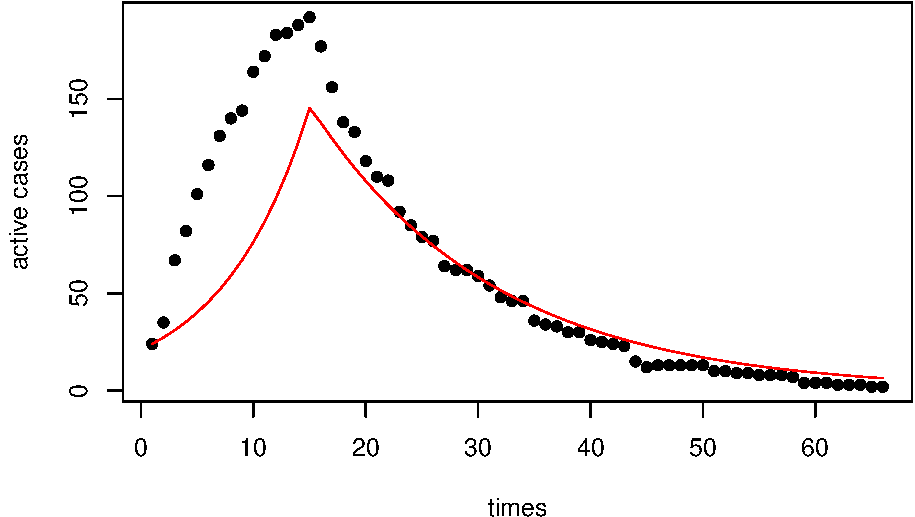
\includegraphics{math-4190_files/figure-latex/unnamed-chunk-9-1.pdf}

\section{}\label{section}

\chapter{A7. Thurs Mar 4: Final project
ideas}\label{a7.-thurs-mar-4-final-project-ideas}

Assignment 7: to be handed in to Brightspace on Tues Mar 9 by 2pm.

\chapter{Final project}\label{final-project}

\begin{itemize}
\tightlist
\item
  Oral presentation - 15\% (week of April 5)
\item
  Written Project - 50\% (due Monday April 12 at 9am)
\end{itemize}

The main focus of the second half of MATH 4190 is the final project. You
are to:

\begin{itemize}
\tightlist
\item
  derive and analyze an original mathematical model,
\item
  extend and analyze an existing mathematical model, or
\item
  explain, recreate and/or produce novel proofs for an existing analysis
  of a mathematical model involving advanced mathematics (i.e., graduate
  level).
\end{itemize}

\section{Written Report}\label{written-report}

Your written report should consist of four sections: Introduction,
Model, Results, and Discussion (for more details see below). You must
appropriately acknowledge results and models that are not your own work.
Your written report must be no more than 10 pages (excluding references,
figures, and appendices) and written in Latex. If you have more than 10
pages of important content, then you should choose to place some of this
content in an Appendix.

Some advice: - Start simple. Start with a model that you are confident
that you will be able to produce some results for. When you fully
understand simpler versions of your model, gradually add in more
complexity. This prevents you from tackling a project this is `too hard'
and not getting any results. - Be concise. A good project is
thoughtfully put together -- it does not necessarily need to be overly
complex or long.

Guidelines for each section of the final project:

\subsection{Introduction}\label{introduction}

\begin{itemize}
\tightlist
\item
  Describe the general question/problem of interest.
\item
  Describe the real-world application in language that is accessible to
  a reader without prior knowledge of the application.
\item
  Summarize relevant previous research from the scientific literature
  (i.e., scholarly journals and books) and clearly place the project
  within the context of what has already been done. Remember to cite
  modeling articles, not just articles that describe the details of your
  applied system.
\item
  Don't focus your literature research to narrowly. For example, if you
  project is on `moose-wolf population dynamics' consider also the
  literature on predator-prey dynamics, which may contain mathematically
  equivalent model formulations.
\item
  Concisely state the main objective, hypothesis or question of the
  project.
\item
  Usually ends with a paragraph describing how the problem will be
  solved, i.e., the type of model and the type of analysis.
\end{itemize}

\subsection{Model}\label{model}

\begin{itemize}
\tightlist
\item
  Your model should be a dynamical system. The model cannot be an
  autonomous linear system of differential equations or difference
  equations because the analysis of such a model is too simple. You may
  however, consider a simplification of the model you are interested in
  that is an autonomous linear system of equations, if it helps you to
  understand the non-linear or non-autonomous system of interest.
\item
  Provide all details of the model to be analyzed. Define all the model
  parameters, variables, provide their word definitions and state their
  units. Provide the complete system of equations that comprises the
  model. If appropriate provide a table of parameter values (and
  references if literature sources are used to justify choices of
  parameter values).
\item
  You should describe the assumptions of your model.
\item
  You should provide enough detail that your model is reproducible. This
  may mean that you need to appendicize some material.
\item
  Consider including a diagram that communicates the interactions
  present in your model. This is often useful.
\end{itemize}

\subsection{Results}\label{results}

\begin{itemize}
\tightlist
\item
  If possible, consider special cases of your model that yield
  analytical solutions such as equilibria and local stability
  conditions.
\item
  If it is possible to solve for the equilibrium values and/or to
  determine the local stability of equilibria for your model you must do
  so.
\item
  Usually the results section of a MATH 4190 project includes numerical
  solutions for the main model of interest.
\item
  You may wish to summarize how numerical results for your model change
  depending on the parameter values used.
\item
  Depending on your project, you may wish to explore different types of
  more advanced analyses, i.e.~perturbation analysis, sensitivity and
  uncertainty analysis, stochastic simulations based on the Gillespie
  algorithm, bifurcation diagrams, analysis of periodic systems, and
  model validation.
\item
  You do not need to hand in your code. If your numerical methods are
  complex or non-standard you may wish to provide your pseudo-code in an
  Appendix.
\item
  Your results should include at least 1 figure that is fully labeled
  and contains a figure caption.
\item
  Your results section does not need to include every analysis that you
  have done. Your results section should be logically organized and this
  may mean omitting analyses that `didn't work out' or you judge to be
  less important given later results that you were able to achieve. Your
  results should be appropriate given the question/hypothesis that you
  described in the Introduction.
\end{itemize}

\subsection{Discussion}\label{discussion}

\begin{itemize}
\tightlist
\item
  Interpret your results in terms of the main question/hypothesis.
\item
  Towards the beginning of the Discussion, typically there is a section
  that reiterates the highlights of the results section.
\item
  Your discussion should describe whether your results matched what was
  expected or not. Are your results consistent with other similar
  studies?
\item
  You should interpret your results in the context of the applied
  problem, i.e., what does a stability condition suggest in terms of the
  practical management of a system?
\item
  How did your assumptions affect your results?
\item
  Do your results suggest any avenues for future research?
\item
  Highlight what is novel about your work.
\end{itemize}

You are to provide a complete bibliography of literature cited. You can
choose to use the referencing style of any scholarly scientific journal
or any of the preset options from Bibtex. The referencing style you use
must be consistent throughout.

\section{Oral report}\label{oral-report}

The content of your oral report should be similiar to the written
report.

I am here to help! Please let me know if you have any questions.

For writing tips, you may consider: (1)
\href{https://m3challenge.siam.org/sites/default/files/uploads/siam-guidebook-final-press.pdf}{Bliss
et al. 2014} (p42-44); (2)
\href{http://matryoshka.org/2012/07/13/how-to-write-a-paper-people-will-cite/}{``How
to write a theoretical ecology paper that people will cite''}; or (3)
\href{https://video.mbi.ohio-state.edu/video/player/?id=4775\&title=Webinar\%3A\%20How\%20to\%20Write\%20a\%20Modelling\%20Paper}{Webinar:
How to write a modelling paper}

\end{document}
